\documentclass[aspectratio=169, 11pt]{beamer}

% ── Theme & Colors ──────────────────────────────────────────────
\usetheme{Madrid}
\usecolortheme{default}
\definecolor{darkblue}{RGB}{0,51,102}
\definecolor{lightblue}{RGB}{51,122,183}
\definecolor{darkgreen}{RGB}{34,139,34}
\definecolor{highlight}{RGB}{220,50,47}
\setbeamercolor{structure}{fg=darkblue}
\setbeamercolor{frametitle}{bg=darkblue, fg=white}
\setbeamercolor{block title}{bg=lightblue, fg=white}
\setbeamercolor{block body}{bg=lightblue!10}
\setbeamercolor{block title alerted}{bg=highlight, fg=white}
\setbeamercolor{block body alerted}{bg=highlight!10}
\setbeamertemplate{navigation symbols}{}
\setbeamertemplate{footline}[frame number]

% ── Packages ────────────────────────────────────────────────────
\usepackage{amsmath, amssymb}
\usepackage{booktabs}
\usepackage{csquotes}
\usepackage{tikz}
\usetikzlibrary{arrows.meta, positioning, decorations.pathreplacing}
\usepackage{graphicx}
\usepackage{xcolor}

% ── Macros ──────────────────────────────────────────────────────
\newcommand{\vx}{\mathbf{x}}
\newcommand{\vz}{\mathbf{z}}
\newcommand{\PP}{\mathcal{P}}
\newcommand{\R}{\mathbb{R}}
\DeclareMathOperator*{\argmin}{arg\,min}

% ── Title ───────────────────────────────────────────────────────
\title[CPP Counterfactuals]{%
  Certified Polyhedral Projection\\[4pt]
  for Counterfactual Explanations}
\subtitle{Generating Valid, Proximal, and Robust Counterfactuals\\via Preimage Approximation}
\author{Gabriele Pintus}
\date{\today}

\begin{document}

% ================================================================
\begin{frame}
  \titlepage
\end{frame}

% ================================================================
\begin{frame}{Outline}
  \tableofcontents
\end{frame}

% ================================================================
\section{Motivation}

% ----------------------------------------------------------------
\begin{frame}{What Are Counterfactual Explanations?}

A classifier labels an input $\vx_0$ as class $l$. We ask:

\begin{block}{Goal}
  Find $\vx'$ classified as a \textbf{different target class} $t$, \textbf{as close as possible} to $\vx_0$.
\end{block}

\bigskip

\textbf{Example (MNIST):} \enquote{What minimal change turns a \textbf{digit 1} into a \textbf{digit 7}?}

\bigskip

\textbf{Desirable properties:}
\begin{enumerate}
  \item \textbf{Validity} -- guaranteed to be classified as the target class
  \item \textbf{Proximity} -- minimal distance to the original input
  \item \textbf{Plausibility} -- stays close to the data manifold
  \item \textbf{Robustness} -- remains valid under small perturbations
\end{enumerate}

\end{frame}

% ----------------------------------------------------------------
\begin{frame}{Why Not Gradient Descent?}

Standard methods minimize a loss that trades off distance and target-class confidence:

\begin{alertblock}{Problems}
\begin{itemize}
  \item \textbf{Non-convex} -- gets stuck in local minima
  \item \textbf{No validity guarantee} -- result may sit right at the decision boundary
  \item \textbf{Not robust} -- tiny perturbations can flip the prediction back
\end{itemize}
\end{alertblock}

\bigskip

\begin{center}
\textbf{Our approach:} replace gradient descent\\
with \textcolor{darkgreen}{\textbf{projection onto certified safe regions}}.
\end{center}

\end{frame}

% ================================================================
\section{The CPP Method}

% ----------------------------------------------------------------
\begin{frame}{Core Idea}

\begin{block}{Key Insight}
  Around each training sample we can build a \textbf{convex region} (polytope) where the classifier is \emph{guaranteed} to predict a specific class.

  \bigskip

  Finding a counterfactual = \textbf{projecting onto the nearest such region}.
\end{block}

\bigskip

\begin{itemize}
  \item Projection onto a convex polytope is a \textbf{convex optimization problem}
  \item Convex $\Rightarrow$ \textbf{global optimum}, no local minima
  \item No trade-off hyperparameter $\lambda$ needed
\end{itemize}

\end{frame}

% ----------------------------------------------------------------
\begin{frame}{Two-Phase Architecture}

\begin{columns}[T]
\column{0.48\textwidth}
\begin{block}{Phase I -- Offline: Build Atlas}
  For each training sample $\mathbf{c}_i$ of class $t$:
  \begin{enumerate}
    \item Consider a small region around $\mathbf{c}_i$ (an $\varepsilon$-ball)
    \item Use \textbf{LiRPA} to find linear constraints that \emph{certify} the classifier predicts $t$ throughout this region
    \item Store the resulting \textbf{certified polytope} $\PP_i$
  \end{enumerate}
  \medskip
  $\Rightarrow$ Every point inside $\PP_i$ is \textbf{guaranteed class $t$}
\end{block}

\column{0.48\textwidth}
\begin{block}{Phase II -- Online: Query}
  Given a query $\vx_0$:
  \begin{enumerate}
    \item Use a \textbf{spatial index} (BVH) to quickly find nearby polytopes
    \item \textbf{Project} $\vx_0$ onto each candidate polytope (convex QP)
    \item Return the \textbf{closest} valid projection
  \end{enumerate}
  \medskip
  $\Rightarrow$ Result is \textbf{certifiably} classified as target
\end{block}
\end{columns}

\end{frame}

% ================================================================
\section{How It Works}

% ----------------------------------------------------------------
\begin{frame}{Step 1: Certifying Regions with LiRPA}

\textbf{LiRPA} (Linear Relaxation based Perturbation Analysis) gives us \textbf{linear lower bounds} on the network within a small region around each sample.

\medskip

\begin{center}
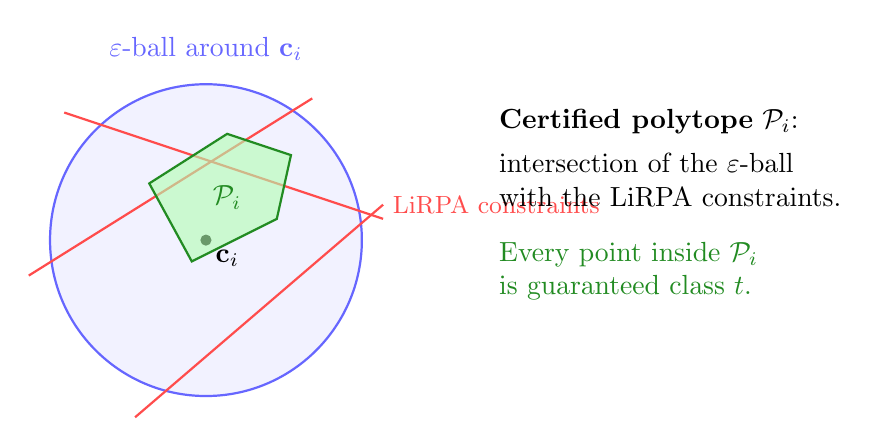
\begin{tikzpicture}[scale=0.9]
  % Epsilon ball
  \draw[thick, blue!60, fill=blue!5] (0,0) circle (2.2cm);
  \node[blue!60, above] at (0, 2.4) {$\varepsilon$-ball around $\mathbf{c}_i$};

  % Center point
  \filldraw[black] (0,0) circle (2pt) node[below right] {$\mathbf{c}_i$};

  % Halfspaces (lines)
  \draw[thick, red!70] (-2.5, -0.5) -- (1.5, 2.0);
  \draw[thick, red!70] (-1.0, -2.5) -- (2.5, 0.5);
  \draw[thick, red!70] (-2.0, 1.8) -- (2.5, 0.3);

  \node[red!70, right, font=\small] at (2.5, 0.5) {LiRPA constraints};

  % Certified polytope (intersection)
  \fill[green!30, opacity=0.6] (-0.2, -0.3) -- (1.0, 0.3) -- (1.2, 1.2) -- (0.3, 1.5) -- (-0.8, 0.8) -- cycle;
  \draw[thick, darkgreen] (-0.2, -0.3) -- (1.0, 0.3) -- (1.2, 1.2) -- (0.3, 1.5) -- (-0.8, 0.8) -- cycle;

  \node[darkgreen, font=\bfseries] at (0.3, 0.6) {$\PP_i$};

  % Result description
  \node[right, align=left] at (4, 0.5) {
    \textbf{Certified polytope} $\PP_i$:\\[4pt]
    intersection of the $\varepsilon$-ball\\
    with the LiRPA constraints.\\[8pt]
    \textcolor{darkgreen}{Every point inside $\PP_i$}\\
    \textcolor{darkgreen}{is guaranteed class $t$.}
  };
\end{tikzpicture}
\end{center}

\smallskip

The collection of all polytopes for a class forms the \textbf{Certified Atlas}.

\end{frame}

% ----------------------------------------------------------------
\begin{frame}{Step 2: Fast Search with BVH}

With ${\sim}1000$ polytopes per class, checking all of them is too slow.

\medskip

\begin{columns}[T]
\column{0.55\textwidth}
\begin{block}{Bounding Volume Hierarchy}
\begin{itemize}
  \item Organize polytopes in a \textbf{binary tree} of bounding boxes
  \item \textbf{Branch-and-bound}: skip subtrees that can't contain a closer match
  \item Same result as exhaustive search
\end{itemize}
\end{block}

\medskip

\textbf{Result on MNIST ($d = 784$):}
\begin{itemize}
  \item Exhaustive: $\sim$1000 projections/query
  \item BVH: $\sim$2--5 projections/query
  \item \textbf{$200$--$500\times$ speedup}
\end{itemize}

\column{0.40\textwidth}
\vspace{0.5cm}
\begin{center}
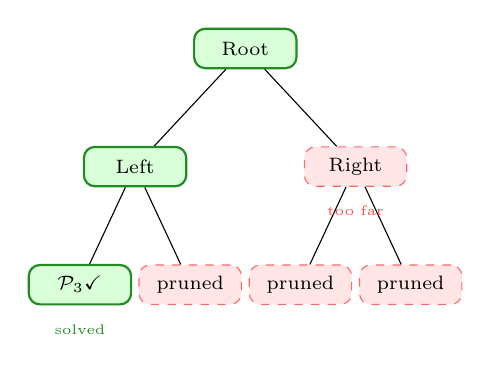
\begin{tikzpicture}[
  every node/.style={draw, rounded corners, minimum width=1.3cm, minimum height=0.5cm, font=\scriptsize},
  prune/.style={draw=red!60, fill=red!10, dashed},
  visit/.style={draw=darkgreen, fill=green!15, thick},
  level 1/.style={sibling distance=2.8cm},
  level 2/.style={sibling distance=1.4cm}
]
  \node[visit] (root) {Root}
    child {
      node[visit] (L) {Left}
      child { node[visit] (LL) {$\PP_3$\checkmark} }
      child { node[prune] (LR) {pruned} }
    }
    child {
      node[prune] (R) {Right}
      child { node[prune] (RL) {pruned} }
      child { node[prune] (RR) {pruned} }
    };

  \node[draw=none, below=0.05cm of LL, font=\tiny, darkgreen] {solved};
  \node[draw=none, below=0.05cm of R, font=\tiny, red!70] {too far};
\end{tikzpicture}
\end{center}
\end{columns}

\end{frame}

% ================================================================
\section{Robust Counterfactuals}

% ----------------------------------------------------------------
\begin{frame}{Making Counterfactuals Robust}

A counterfactual at the polytope boundary can be flipped by a tiny perturbation.

\begin{block}{Idea: Erode the Polytope Inward by $\delta$}
  Shrink constraints so that the \textbf{entire ball of radius $\delta$} around the counterfactual stays inside.
\end{block}

\vspace{-2pt}

\begin{center}
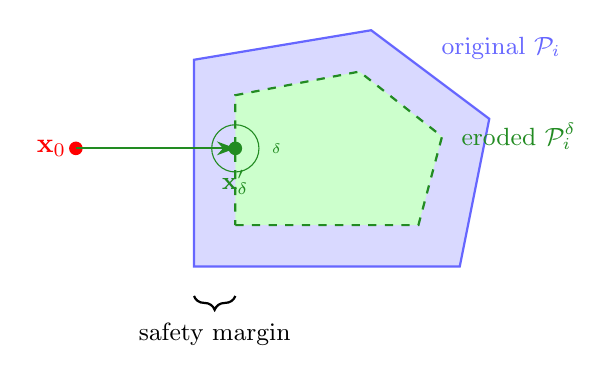
\begin{tikzpicture}[scale=0.75]
  % Original polytope
  \fill[blue!15] (-2,-1.5) -- (2.5,-1.5) -- (3,1) -- (1,2.5) -- (-2,2) -- cycle;
  \draw[thick, blue!60] (-2,-1.5) -- (2.5,-1.5) -- (3,1) -- (1,2.5) -- (-2,2) -- cycle;
  \node[blue!60, font=\small] at (3.2, 2.2) {original $\PP_i$};

  % Eroded polytope
  \fill[green!20] (-1.3,-0.8) -- (1.8,-0.8) -- (2.2,0.7) -- (0.8,1.8) -- (-1.3,1.4) -- cycle;
  \draw[thick, darkgreen, dashed] (-1.3,-0.8) -- (1.8,-0.8) -- (2.2,0.7) -- (0.8,1.8) -- (-1.3,1.4) -- cycle;
  \node[darkgreen, font=\small] at (3.5, 0.7) {eroded $\PP_i^\delta$};

  % Query point
  \filldraw[red] (-4, 0.5) circle (3pt) node[left] {$\vx_0$};

  % Robust CF
  \draw[-{Stealth}, thick, darkgreen] (-4, 0.5) -- (-1.3, 0.5);
  \filldraw[darkgreen] (-1.3, 0.5) circle (3pt);
  \node[darkgreen, below, font=\small] at (-1.3, 0.3) {$\vx'_\delta$};
  \draw[darkgreen, thin] (-1.3, 0.5) circle (0.4cm);
  \node[darkgreen, font=\tiny, right] at (-0.85, 0.5) {$\delta$};

  % Annotation
  \draw[decorate, decoration={brace, amplitude=5pt, mirror}, thick]
    (-2, -2) -- (-1.3, -2) node[midway, below=6pt, font=\small] {safety margin};
\end{tikzpicture}
\end{center}

\begin{itemize}
  \item Larger $\delta$ $\Rightarrow$ more robust, but farther from original
  \item Too large $\delta$ $\Rightarrow$ eroded polytope becomes empty
\end{itemize}

\end{frame}

% ----------------------------------------------------------------
\begin{frame}{Cross-Norm Robustness}

The norm used to build the atlas ($p$) and the robustness norm ($q$) can \textbf{differ}.

Two things must be adjusted:

\bigskip

\textbf{1. Each linear constraint} is pushed inward by $\delta \cdot \|\text{normal}\|_{q^*}$, where $q^*$ is the \textbf{dual} of $q$:

\smallskip
\begin{center}
\begin{tabular}{lccc}
  \toprule
  Robustness norm $q$ & $L_1$ & $L_2$ & $L_\infty$ \\
  \midrule
  Dual norm $q^*$ & $L_\infty$ & $L_2$ & $L_1$ \\
  \bottomrule
\end{tabular}
\end{center}

\bigskip

\textbf{2. The $\varepsilon$-ball} must shrink to accommodate the robustness ball. The cost depends on a \textbf{key norm inequality}:

\[
  \|\vx\|_{p_2} \;\leq\; \|\vx\|_{p_1} \quad\text{for } p_2 > p_1
\]

\begin{itemize}
  \item If $q < p$ (e.g., $L_2$ robustness on $L_\infty$ atlas): the robustness ball \textbf{fits for free} $\Rightarrow$ \textcolor{darkgreen}{\textbf{cheap}}
  \item If $q > p$: the ball must be shrunk by a factor growing with dimension $d$ $\Rightarrow$ \textcolor{highlight}{\textbf{expensive in high $d$}}
\end{itemize}

\end{frame}

% ================================================================
\section{Results}

% ----------------------------------------------------------------
\begin{frame}{Results on MNIST}

\begin{columns}[T]
\column{0.48\textwidth}
\textbf{Setup:}
\begin{itemize}
  \item CNN classifier, 99.2\% accuracy
  \item 10,000 polytopes (1000/class)
  \item 784-dimensional input
\end{itemize}

\bigskip

\textbf{Counterfactual generation:}
\begin{itemize}
  \item \textbf{100\% validity} (by construction)
  \item BVH: \textbf{2--5 projections/query}\\(vs.\ 1000 exhaustive)
  \item 180 counterfactuals evaluated
\end{itemize}

\column{0.48\textwidth}
\begin{center}
\begin{tabular}{lr}
  \toprule
  \textbf{Metric} & \textbf{Mean} \\
  \midrule
  $\ell_2$ distance           & 23.4  \\
  Pixels changed (/784)       & 224   \\
  Sparsity                    & 29\%  \\
  LOF score                   & 1.55  \\
  QP solves (BVH)             & 3.4   \\
  \bottomrule
\end{tabular}
\end{center}

\bigskip

\begin{itemize}
  \item LOF $\approx 1$: counterfactuals look like \textbf{real target-class data}
  \item $\sim$29\% pixels changed: \textbf{moderately sparse}
\end{itemize}
\end{columns}

\end{frame}

% ================================================================
\section{Summary}

% ----------------------------------------------------------------
\begin{frame}{Summary}

\begin{block}{What we did}
\begin{enumerate}
  \item \textbf{Certified Polyhedral Projection} -- counterfactual generation via convex projection instead of gradient descent
  \item \textbf{Provable validity} -- every counterfactual lies inside a certified region
  \item \textbf{Robustness} -- polytope erosion guarantees stability under perturbations, even across different norms
  \item \textbf{Efficiency} -- BVH spatial indexing gives $200$--$500\times$ speedup
\end{enumerate}
\end{block}

\bigskip

\begin{block}{Key advantages over standard methods}
\begin{itemize}
  \item No trade-off hyperparameter $\lambda$
  \item Convex QP $\Rightarrow$ global optimum per polytope
  \item Atlas built once offline, queries are fast
\end{itemize}
\end{block}

\end{frame}

% ----------------------------------------------------------------
\begin{frame}

\begin{center}
  {\Huge\textcolor{darkblue}{Thank You}}

  \bigskip

  {\large Questions?}

  \bigskip\bigskip

  \texttt{github.com/gabrielepintus/PreimageCounterfactualSampling}
\end{center}

\end{frame}

\end{document}
